\begin{exo}
	Dans une étude statistique, on considère une classe de 24 élèves où chaque élève est représenté par une case dans le graphique ci-dessous :

	\begin{center}
		\begin{tikzpicture}[scale=0.7]
			\fill[black!30] (0,0) rectangle (2,4);
			\fill[pattern=north east lines] (0,1) rectangle (1,4);
			\fill[pattern=north east lines] (1,2) rectangle (2,4);
			\fill[pattern=north east lines] (2,3) rectangle (6,4);
			\draw[step=1cm, black, thin] (0,0) grid (6,4);
		\end{tikzpicture}
		\hfill
		\begin{tikzpicture}[scale=0.6, every node/.style={scale=0.9}]
			\draw[fill=black!30] (0,1.2) rectangle (1.5,1.7) node[right, black, midway, xshift=0.9cm] {Garçon};
			\draw[pattern=north east lines] (0,0.3) rectangle (1.5,0.8) node[right, black, midway, xshift=0.9cm] {Demi-pensionnaire};
		\end{tikzpicture}
	\end{center}

	Deux caractères sont étudiés chez les individus de cette étude :
	\begin{itemize}
		\item $G$ : \og{} l'élève est un garçon \fg{} ;
		\item $D$ : \og{} l'élève est demi-pensionnaire \fg{}.
	\end{itemize}

	L'expérience aléatoire consiste à choisir un élève au hasard dans la classe et de regarder la réalisation ou non de ces deux critères.
	\begin{enumerate}
		\item Compléter l'arbre de probabilité ci-dessous.
	\end{enumerate}

	\begin{center}
		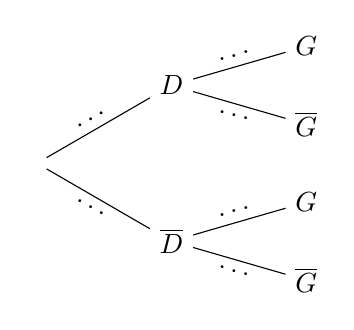
\begin{tikzpicture}[grow=right, sloped, level distance=1.9cm,
				level 1/.style={sibling distance=2.2cm},
				level 2/.style={sibling distance=1.1cm},
				scale=0.9]

			\node {}
			child {node {$\overline{D}$}
					child {node {$\overline{G}$} edge from parent node[below] {\dots}}
					child {node {$G$} edge from parent node[above] {\dots}}
					edge from parent node[below] {\dots}
				}
			child {node {$D$}
					child {node {$\overline{G}$} edge from parent node[below] {\dots}}
					child {node {$G$} edge from parent node[above] {\dots}}
					edge from parent node[above] {\dots}
				};
		\end{tikzpicture}
	\end{center}

	\begin{enumerate}[resume]
		\item Donner par lecture directe la valeur des probabilités suivantes :
		      \[
			      P(D),\ P_{D}(G)\ \text{et}\ P_{\overline{D}}(\overline{G})
		      \]

		\item Calculer la probabilité de l'événement $G \cap \overline{D}$.
		\item Calculer la probabilité que l'élève choisi soit une fille demi-pensionnaire.
		\item Sachant que l'élève choisi est un garçon, quelle est la probabilité qu'il soit demi-pensionnaire ?
	\end{enumerate}
\end{exo}
